%!TEX root = ../template.tex
%%%%%%%%%%%%%%%%%%%%%%%%%%%%%%%%%%%%%%%%%%%%%%%%%%%%%%%%%%%%%%%%%%%%
%% chapter5.tex
%% NOVA thesis document file
%%
%% Chapter with lots of dummy text
%%%%%%%%%%%%%%%%%%%%%%%%%%%%%%%%%%%%%%%%%%%%%%%%%%%%%%%%%%%%%%%%%%%%
\chapter{Evaluation}
\label{cha:evaluation}

The following chapter reports on the experimental work performed in order to study both the performance of the implemented replication module and the executability and the performance melhories to the introduction of a cache server.

To answer the questions presented at the beginning of this work, we need to conduct an evaluation of

%%-------------------------------------------------------------------
%%	5. - Motivation
%%-------------------------------------------------------------------
\section{Motivation}
\label{sec:eval_motivation}

\textbf{TOPICS :}
\begin{itemize}
	\item Benchmark the iCBD-Replication Module
	\item Assert the performance gained by storing iMI closer to client workstations
\end{itemize}

%https://stackoverflow.com/questions/1198691/testing-io-performance-in-linux
%https://dl.acm.org/citation.cfm?id=1367829.1367831

%https://github.com/axboe/fio
%https://github.com/giantswarm/filesystem-benchmark

\section{Metodology}
\label{sec:eval_method}

\section{Experimental Setup}
\label{sec:eval_exp_setup}

\begin{table}[htpb]
\centering
\begin{tabular}{lcc}
\hline
                             & \textbf{FCT NOVA}          & \textbf{Reditus}              \\ \hline
\textit{\textbf{Servers}}    & 2x HP ProLiant DL380 Gen9 & 2 x HP ProLiant DL380 Gen9    \\
\textit{\textbf{Switch}}     & HPE Flexfabric 5700 jg898a & HPE Flexfabric 5700 jg898a    \\
\textit{\textbf{Disk Array}} & HPE MSA 2040 SAN Storage   & N/A - (Storage on the Server) \\
\textit{\textbf{Networking}} & 10 Gbps (between servers)  & 10 Gbps (between servers)     \\ \hline
\end{tabular}
\caption{Physical infrastructure of the FCT NOVA and SolidNetworks sites}
\end{table}

\begin{table}[htpb]
\centering
\begin{tabular}{ll}
\textit{\textbf{CPU}}             & 2x Intel Xeon E5-2670 v3 @ 2.30GHz        \\
\textit{\textbf{Memory}}          & 128 GB                                    \\
\textit{\textbf{Controller Type}} & 12Gb/s SAS                                \\
\textit{\textbf{Ethernet}}        & 2 ports at 10 Gbps plus 4 ports at 1 Gbps \\
\textit{\textbf{Hypervisor}}      & VMware ESXi, 6.5.0, 4564106              
\end{tabular}
\caption{Specifications of one HP ProLiant DL380 Gen9 host}
\end{table}

\begin{table}[htpb]
\centering
\begin{tabular}{ll}
\textit{\textbf{Controllers}}    & 2 MSA 2040 SAS                          \\
\textit{\textbf{Total Capacity}} & 7.2 TB                                  \\
\textit{\textbf{Disks}}          & 12 HP SAS 600GB 10k Rpms                \\
\textit{\textbf{Host interface}} & 8 12Gb/sec SAS ports (4 per controller) \\
\textit{\textbf{Ethernet}}       & 2 ports at 1 Gbps (1 per controller)   
\end{tabular}
\caption{Specifications of the HPE MSA 2040 SAN Storage}
\end{table}


Unless stated otherwise, all tests were executed ten times removing the best and worst result. The final result is the average of the remaining values. 
%Throughput results are presented in Transactions per Minute (TPM).

%%-------------------------------------------------------------------
%%	5. - Functional Testing
%%-------------------------------------------------------------------
\section{Replication Testing}
\label{sec:eval_rep_functional_testing}

\textbf{TOPICS :}
\begin{itemize}
	\item Replication with rsync (100 / 1000 mbps)
	\item Replication with iCBD-Replication - Plain Sockets and No Compression (100 / 1000 mbps)
	\item Replication with iCBD-Replication - Plain Sockets and LZ4 Compression (100 / 1000 mbps)
	\item Replication with iCBD-Replication - Plain Sockets and zlib Compression (100 / 1000 mbps)
	\item Replication with iCBD-Replication - Plain Sockets and snappy Compression (100 / 1000 mbps)
	\item Replication with iCBD-Replication - SSH and No Compression (100 / 1000 mbps)
\end{itemize}

%https://stackoverflow.com/questions/5357601/whats-the-difference-between-unit-tests-and-integration-tests

% Unit Test Python
%https://docs.python.org/2/library/unittest.html

%Memory profile of the module
%https://pypi.python.org/pypi/memory_profiler

%%-------------------------------------------------------------------
%%	5. - Integration Testing
%%-------------------------------------------------------------------
\section{Plataform Testing}
\label{sub:eval_integration_testing}

\begin{figure}[htbp]
	\centering
	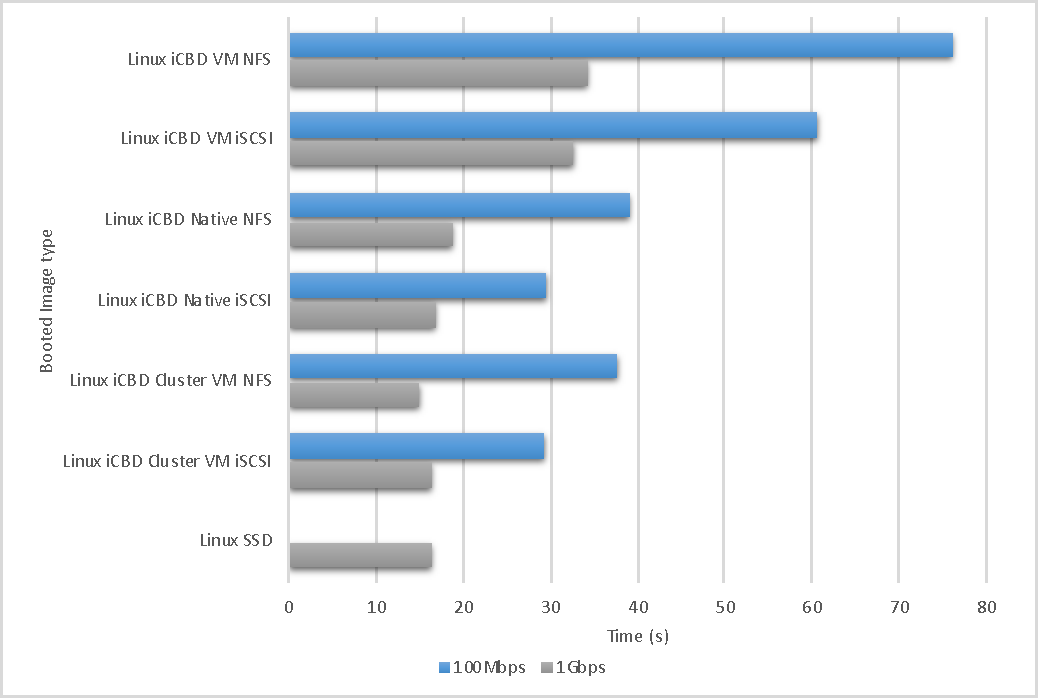
\includegraphics[height=4in]{cap5_boot_imgs}
	\caption{Boot time from iCBD-imgs VM}
	\label{fig:boot_imgs}
\end{figure}

\begin{figure}[htbp]
	\centering
	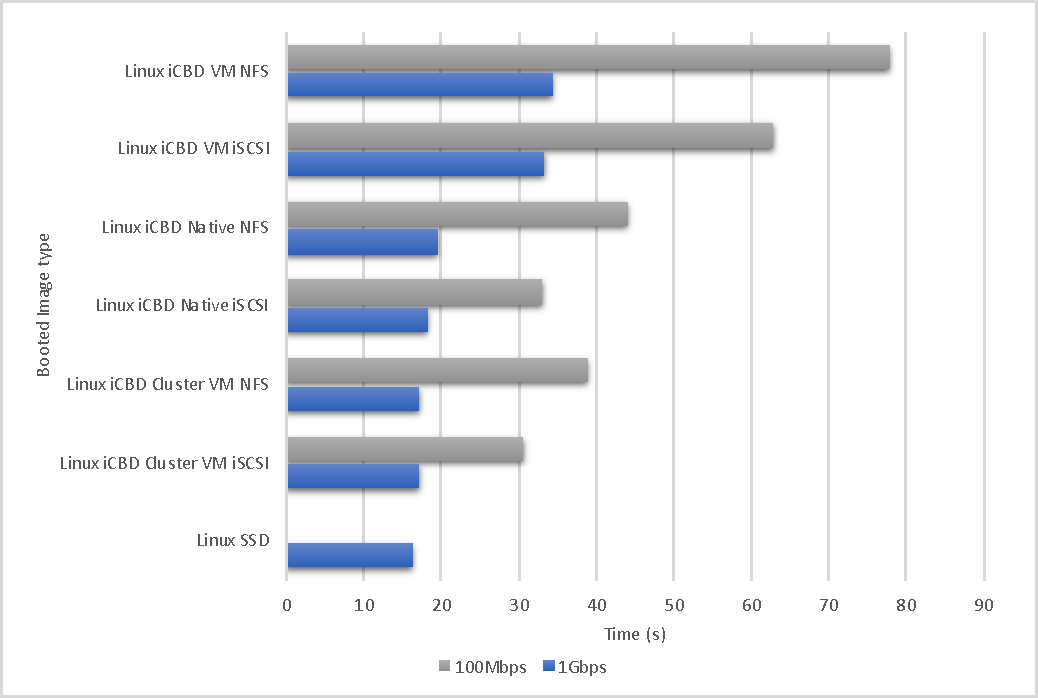
\includegraphics[height=4in]{cap5_boot_cache}
	\caption{Boot time from iCBD-Cache02}
	\label{fig:boot_cache}
\end{figure}


\textbf{TOPICS :}
\begin{itemize}
	\item benchmarking 
	\item Boot time Lab PC
	\item Boot time iCBD VM in Cluster
	\item Boot time iCBD in Lab PC (100 / 1000 mbps) iCBD-Imgs VM
	\item Boot time iCBD in Lab PC (100 / 1000 mbps) iCBD-Cache
\end{itemize}